\documentclass[conference]{IEEEtran}
\IEEEoverridecommandlockouts
\renewcommand\IEEEkeywordsname{Keywords}

\usepackage[utf8]{inputenc}
\usepackage[T1]{fontenc}
\usepackage[american]{babel}
\usepackage{cite}
\usepackage{amsmath,amssymb,amsfonts}
\usepackage{graphicx}
\usepackage{textcomp}
\usepackage{booktabs}
\usepackage{multirow}
\usepackage{bm}
\usepackage{xcolor}
\usepackage{scalerel}
\usepackage{tikz}
\usetikzlibrary{svg.path}
\usepackage[bookmarks=false]{hyperref}

\definecolor{orcidlogocol}{HTML}{A6CE39}
\tikzset{
  orcidlogo/.pic={
    \fill[orcidlogocol] svg{M256,128c0,70.7-57.3,128-128,128C57.3,256,0,198.7,0,128C0,57.3,57.3,0,128,0C198.7,0,256,57.3,256,128z};
    \fill[white] svg{M86.3,186.2H70.9V79.1h15.4v48.4V186.2z}
                 svg{M108.9,79.1h41.6c39.6,0,57,28.3,57,53.6c0,27.5-21.5,53.6-56.8,53.6h-41.8V79.1z M124.3,172.4h24.5c34.9,0,42.9-26.5,42.9-39.7c0-21.5-13.7-39.7-43.7-39.7h-23.7V172.4z}
                 svg{M88.7,56.8c0,5.5-4.5,10.1-10.1,10.1c-5.6,0-10.1-4.6-10.1-10.1c0-5.6,4.5-10.1,10.1-10.1C84.2,46.7,88.7,51.3,88.7,56.8z};
  }
}

\newcommand\orcid[1]{\href{https://orcid.org/#1}{\mbox{\scalerel*{

\begin{tikzpicture}[yscale=-1,transform shape]
\pic{orcidlogo};
\end{tikzpicture}
}{|}}}}

\makeatletter
\let\old@ps@headings\ps@headings
\let\old@ps@IEEEtitlepagestyle\ps@IEEEtitlepagestyle
\def\confheader#1{%
\def\ps@headings{%
\old@ps@headings%
\def\@oddhead{\strut\hfill#1\hfill\strut}%
\def\@evenhead{\strut\hfill#1\hfill\strut}%
}%
\def\ps@IEEEtitlepagestyle{%
\old@ps@IEEEtitlepagestyle%
\def\@oddhead{\strut\hfill#1\hfill\strut}%
\def\@evenhead{\strut\hfill#1\hfill\strut}%
}%
\ps@headings%
}
\makeatother

\confheader{11th Workshop on Communication Networks and Power Systems (WCNPS 2026)}

\begin{document}

\title{Evaluation of Indices for Monitoring the Voltage Stability Margin of Power Systems}

\author{\IEEEauthorblockN{Gonçalo Fontenele \orcid{0009-0008-1378-1420}\IEEEauthorrefmark{1},
Leonardo Rafael Bergonci Campos\IEEEauthorrefmark{1},
Murilo E. C. Bento\IEEEauthorrefmark{1}}
\IEEEauthorblockA{\IEEEauthorrefmark{1}Department of Electrical Engineering, Federal University of Rio de Janeiro\\
Rio de Janeiro, RJ 21941-909, Brazil\\
Email: goncalogfb@poli.ufrj.br, bergoncileo@gmail.com, murilobento@poli.ufrj.br}}

\IEEEpubid{\makebox[\columnwidth]{Copyright Notice}\hspace{\columnsep}\makebox[\columnwidth]{}}
\maketitle

\begin{abstract}
Voltage stability assessment is essential for secure power-system operation under stressed loading conditions. This paper presents an open-source Python framework based on Pandapower for static loadability analysis and the evaluation of Voltage Stability Indices (VSIs). The framework applies successive load increments, distributed generation redispatch, and adaptive backtracking to estimate the Maximum Loading Point (MLP). The IEEE 30-bus ANAREDE equivalent is used as the reference system. Five VSIs, FVSI, $L_{mn}$, NLSI, NVSI, and the L-Index, are evaluated throughout the loadability trajectory, and the similarity among the branch-based indices is quantified using Spearman rank correlation. In addition, N-1 line contingencies are assessed with generator reactive-power limits enforced through PV-to-PQ conversion. The results show that some line-based indices provide highly similar rankings, while the nodal L-Index offers complementary information on bus vulnerability. The contingency analysis further demonstrates that the intact-network margin alone does not characterize the most restrictive operating condition.
\end{abstract}

\begin{IEEEkeywords}
Power Systems, Voltage Stability, Loadability Analysis, Voltage Stability Indices, Pandapower, ANAREDE, N-1 Contingency.
\end{IEEEkeywords}

\section{Introduction}
\label{sec:introduction}

The evolution of power systems has increased the complexity of maintaining secure operation. Growing uncertainty in demand, large-scale integration of renewable generation, equipment outages, extreme weather events, and greater dependence on monitoring and communication infrastructures can push transmission systems closer to their operating limits \cite{Bhusal2020,Pastrana2025,Rifat2025,Manias2024}. Under these conditions, voltage stability becomes a relevant security constraint, particularly when transmission networks and generators are no longer able to provide the reactive-power support required by the load \cite{Hatziargyriou2021,kundur1994power}.

The Maximum Loading Point (MLP) and the associated Voltage Stability Margin (VSM) are commonly determined through loadability studies such as Continuation Power Flow (CPF) \cite{Ajjarapu1992}. Commercial tools such as ANAREDE provide robust procedures for estimating this limit \cite{cepel2009anarede}. However, repeatedly calculating a complete loadability boundary is not always appropriate for monitoring applications. Voltage Stability Indices (VSIs) provide scalar quantities that can be evaluated from electrical states and used to identify stressed transmission corridors or vulnerable buses \cite{modarresi2016comprehensive}. Their potential use in monitoring is reinforced by improved system observability from Phasor Measurement Units (PMUs) and wide-area measurement infrastructures \cite{Pierrou2024,Su2018,Pourbagher2022}.

A large number of VSIs has been proposed using line flows, bus voltages, network equivalents, and admittance-matrix formulations. Although these indices are often interpreted through threshold values close to unity, their mathematical structures differ substantially. Consequently, they may not provide the same ranking of critical elements as the operating point approaches collapse. In addition, the VSM itself depends on the base operating condition, direction of load growth, generation redispatch, reactive-power availability, and network topology \cite{Bento2018b}. These dependencies make it important to evaluate the indices together with an explicit loadability reference rather than interpreting isolated VSI values.

This work addresses this issue through an open-source framework that combines a step-refined loadability search with post-processing of five established VSIs. The IEEE 30-bus ANAREDE equivalent is used throughout the study so that the same electrical model can support validation, VSI comparison, and contingency assessment. The contributions are: (i) cross-comparison of the Python electrical model with ANAREDE; (ii) reproduction of the reference loadability boundary through adaptive step refinement and distributed generation dispatch; (iii) comparative evaluation of FVSI, $L_{mn}$, NLSI, NVSI, and the L-Index along the loading trajectory; (iv) quantitative comparison of branch-based VSI rankings using Spearman correlation; and (v) extension of the analysis to N-1 line contingencies with generator reactive-power limits enforced.

\section{Theoretical Background}
\label{sec:background}

\subsection{Voltage Stability}

Voltage stability is the ability of a power system to maintain acceptable bus voltages after disturbances or gradual changes in operating conditions \cite{kundur1994power}. Large-disturbance voltage stability is associated with severe events such as transmission or generation outages, whereas small-disturbance voltage stability concerns the ability of the system to respond to gradual changes such as load growth. The present study focuses primarily on static voltage stability under progressive loading, while the N-1 assessment introduces topological disturbances to evaluate how the available static margin changes after outages.

As the loading level increases, the power-flow equations approach a limiting operating point associated with a saddle-node bifurcation. At this point, the Jacobian matrix becomes singular and the conventional Newton--Raphson method can no longer obtain a feasible high-voltage solution \cite{cutsem2007voltage}. The resulting loss of solvability is used in this work as the numerical indicator of the static loading boundary.

\subsection{PV Curve}

The PV curve relates active-power demand to bus-voltage magnitude. Starting from the base operating point, increasing system loading generally causes a progressive reduction in voltage until the MLP is reached. The difference between the loading at the base case and at the MLP defines the available static loadability margin. Figure~\ref{fig:curva_pv} illustrates this behavior.

\begin{figure}[!t]
    \centering
    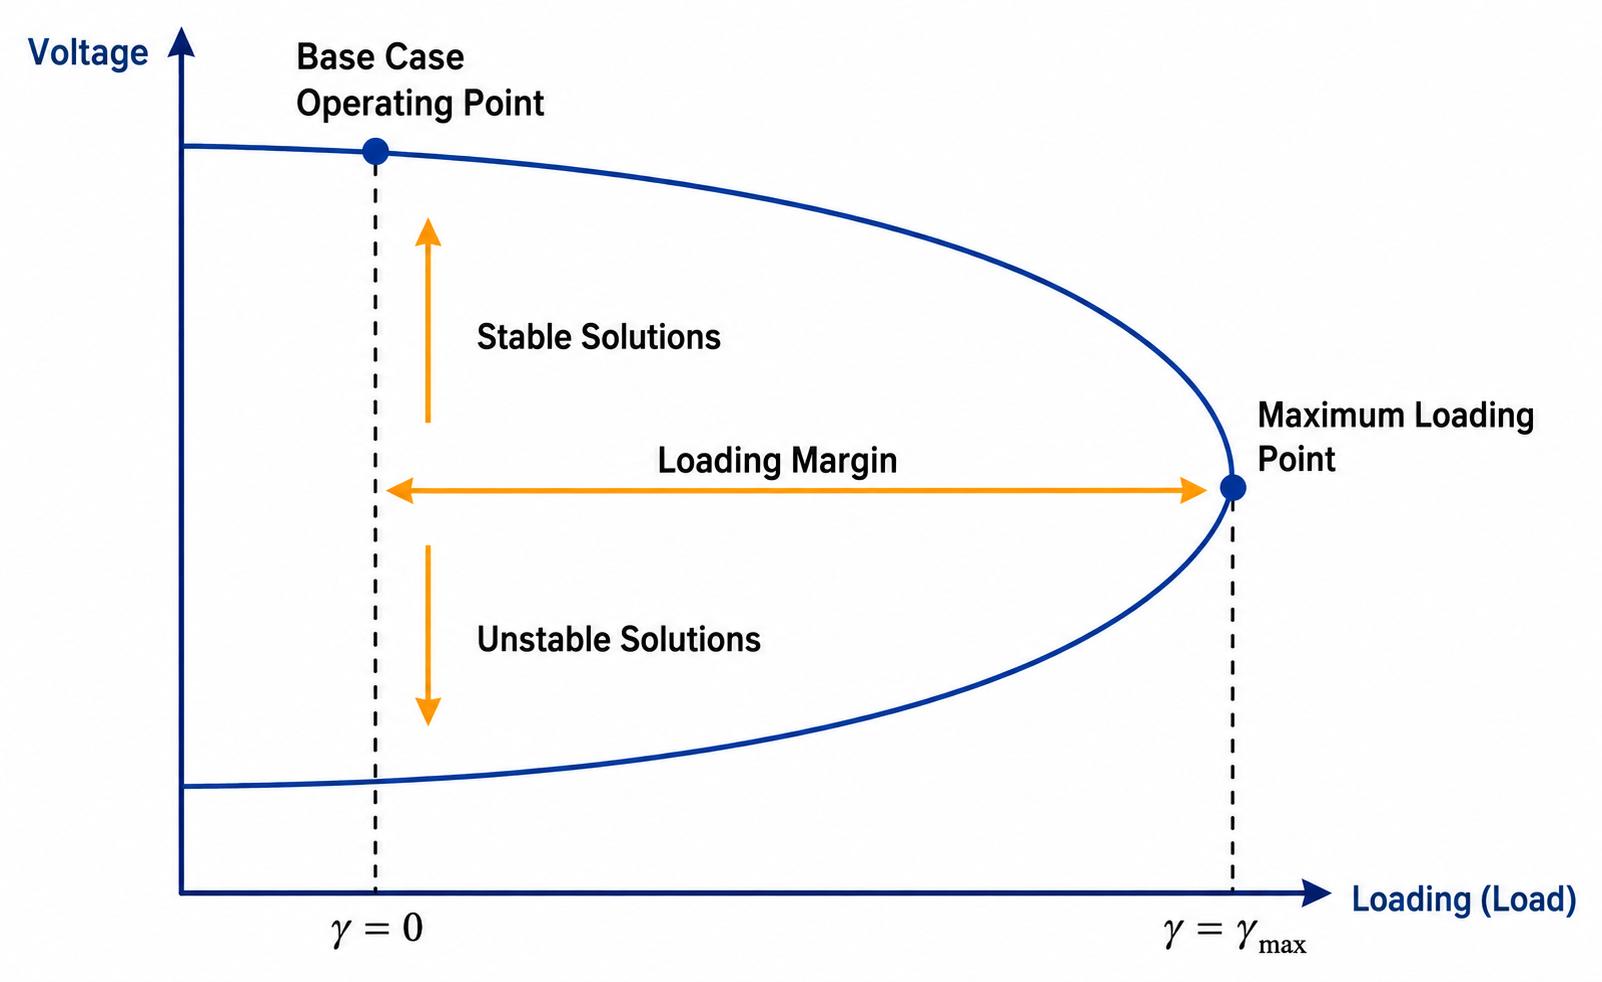
\includegraphics[width=0.82\linewidth]{figures/curva_pv.png}
    \caption{Typical PV curve and Maximum Loading Point \cite{jaquelineresende2007}.}
    \label{fig:curva_pv}
\end{figure}

The PV trajectory is particularly useful as a reference for VSI assessment because it provides an explicit measure of proximity to the loadability boundary. An index intended for monitoring should therefore be interpreted not only by its absolute value but also by how consistently it evolves as the system moves from the base operating point toward the MLP.

\subsection{Review of Voltage Stability Indices}

Voltage Stability Indices (VSIs) are scalar metrics used to quantify the degree of proximity of an electrical system to voltage collapse, reflecting the network's capacity to sustain adequate voltage levels under different loading conditions. Although each index adopts its own formulation and criteria, the general interpretation places them on a scale where values close to zero indicate safe operation and values close to one signal impending collapse. Five VSIs are evaluated in this work. FVSI, $L_{mn}$, NLSI, and NVSI are branch-oriented indices, whereas the L-Index provides a nodal measure based on the network admittance matrix \cite{modarresi2016comprehensive}. For a branch connecting sending bus $i$ to receiving bus $j$, the Fast Voltage Stability Index (FVSI) is written as \cite{musirin2002}

\subsubsection{FVSI (Fast Voltage Stability Index)}
The FVSI is derived from the quadratic form of the power flow equations for a radial line, evaluating the proximity to the point where the equation ceases to have a real solution. Thus, the index expresses how close the system is to violating the discriminant condition $\geq 0$. Values close to 1 indicate that the reactive component of the load at the receiving bus is imposing significant stress on the line. Values greater than 1 indicate that one of the buses connected to the line may face a significant voltage drop, which could lead to a system collapse \cite{musirin2002}. 

For a line connecting bus $i$ (sending) to bus $j$ (receiving), it can be written as:
\begin{equation}
FVSI_{ij} = \frac{4 Z_{ij}^2 Q_j}{V_i^2 X_{ij}} \le 1.0
\end{equation}

\subsubsection{$L_{mn}$ (Line Stability Index)}
The $L_{mn}$ index utilizes the same concept as the FVSI regarding the requirement that the discriminant must be greater than or equal to zero to ensure stability, but it explicitly incorporates the angular dependence between the terminal voltages of the line. It evaluates the role of phase angle displacement and series impedance on stability. Lines with large power flows or heavily loaded lines tend to display small sine values in the denominator, amplifying the index.

Considering the line impedance angle $\theta$ and the angular displacement $\delta = \theta_i - \theta_j$ \cite{moghavvemi98}:
\begin{equation}
L_{mn} = \frac{4 X_{ij} Q_j}{(V_i \sin(\theta - \delta))^2} \le 1.0
\end{equation}

\subsubsection{NLSI (Novel Line Stability Index)}
Proposed to consider the influence of both active and reactive power on collapse, the NLSI expresses the weighted sum of $P$ and $Q$ as a function of the line components $R$ and $X$ \cite{YazdanpanahGoharrizi2007}:
\begin{equation}
NLSI_{ij} = \frac{R_{ij} P_j + X_{ij} Q_j}{0.25 V_i^2} \le 1.0
\end{equation}

\subsubsection{NVSI (New Voltage Stability Index)}
The NVSI uses the apparent power of the load, simultaneously capturing the effects of $P_j$ and $Q_j$. Because its denominator contains the term ($2 Q_j X_{ij} - V_i^2$), the index exhibits high sensitivity to voltage drops: as $V_i$ decreases, the denominator approaches zero, and the NVSI grows rapidly \cite{kanimozhi2013novel}:
\begin{equation}
NVSI_{ij} = \frac{2 X_{ij} S_j}{2 Q_j X_{ij} - V_i^2} \le 1.0
\end{equation}

\subsubsection{L-Index (Bus Index)}
Finally, the L-Index is a bus-oriented indicator that utilizes the hybrid admittance matrix $F$, derived from the $Y_{bus}$ matrix. It measures the distance to collapse for each load bus $j$ \cite{kessel}:

\begin{equation}
L_j = \left| 1 - \sum_{i \in G} F_{ji} \frac{V_i}{V_j} \right|
\end{equation}
Where $G$ is the set of generation buses and matrix $F = -[Y_{LL}]^{-1}[Y_{LG}]$.

\section{Tool Development and Validation}
\label{sec:tool}

A Python tool was developed using Pandapower to represent the reference network, execute the loadability analysis, store the complete converged trajectory, and calculate the VSIs in post-processing. Before applying the loadability procedure, the IEEE 30-bus base case was cross-compared with ANAREDE to verify that the Python representation reproduces the reference electrical state with acceptable consistency.

Table~\ref{tab:comp_tensao} compares voltage magnitudes and angles for representative buses. Exact agreement is obtained at the reference, PV, and synchronous-compensator buses included in the table. The largest difference among the selected load buses is 0.029 pu in voltage magnitude at Bus 30 and $0.5^\circ$ in voltage angle at Bus 12. These differences indicate close agreement in the general voltage profile while also showing that both models should not be treated as numerically identical at every bus.

\begin{table}[!t]
\centering
\caption{Voltage and Angle Comparison: Python vs. ANAREDE}
\label{tab:comp_tensao}
\resizebox{\columnwidth}{!}{
\begin{tabular}{llcccccc}
\toprule
\multirow{2}{*}{\textbf{Bus}} & \multirow{2}{*}{\textbf{Type}} &
\multicolumn{3}{c}{\textbf{Voltage (pu)}} &
\multicolumn{3}{c}{\textbf{Angle (deg.)}} \\
\cmidrule(lr){3-5}\cmidrule(l){6-8}
 & & \textbf{Py} & \textbf{ANA} & \textbf{Diff} &
\textbf{Py} & \textbf{ANA} & \textbf{Diff} \\
\midrule
1  & Ref  & 1.060 & 1.060 & 0.000 & 0.0   & 0.0   & 0.0 \\
2  & PV   & 1.043 & 1.043 & 0.000 & -5.3  & -5.3  & -0.0 \\
5  & Comp & 1.010 & 1.010 & 0.000 & -14.1 & -14.1 & -0.0 \\
8  & Comp & 1.010 & 1.010 & 0.000 & -11.8 & -11.8 & 0.0 \\
12 & PQ   & 1.034 & 1.057 & -0.023 & -15.4 & -14.9 & -0.5 \\
30 & PQ   & 0.963 & 0.992 & -0.029 & -18.0 & -17.6 & -0.4 \\
\bottomrule
\end{tabular}}
\end{table}

Table~\ref{tab:comp_geracao} compares active and reactive generation. Active generation is reproduced very closely, including a 0.1 MW difference at the slack bus. Reactive-power dispatch exhibits larger differences among synchronous compensators, with the largest representative deviation reaching 17.8 Mvar. The comparison therefore supports consistency of the active-power solution and overall electrical state, while reactive-power allocation remains more sensitive to implementation details and control representation.

\begin{table}[!t]
\centering
\caption{Generation Comparison: Python vs. ANAREDE}
\label{tab:comp_geracao}
\resizebox{\columnwidth}{!}{
\begin{tabular}{llcccccc}
\toprule
\multirow{2}{*}{\textbf{Bus}} & \multirow{2}{*}{\textbf{Type}} &
\multicolumn{3}{c}{\textbf{Active Power (MW)}} &
\multicolumn{3}{c}{\textbf{Reactive Power (Mvar)}} \\
\cmidrule(lr){3-5}\cmidrule(l){6-8}
 & & \textbf{Py} & \textbf{ANA} & \textbf{Diff} &
\textbf{Py} & \textbf{ANA} & \textbf{Diff} \\
\midrule
1  & Slack & 260.9 & 261.0 & -0.1 & -19.2 & -16.5 & -2.7 \\
2  & PV    & 40.0  & 40.0  & 0.0  & 44.9  & 49.6  & -4.7 \\
5  & Comp  & 0.0   & 0.0   & 0.0  & 35.9  & 36.0  & -0.1 \\
8  & Comp  & 0.0   & 0.0   & 0.0  & 28.5  & 37.3  & -8.8 \\
11 & Comp  & 0.0   & 0.0   & 0.0  & 23.8  & 16.2  & 7.6 \\
13 & Comp  & 0.0   & 0.0   & 0.0  & 28.4  & 10.6  & 17.8 \\
\bottomrule
\end{tabular}}
\end{table}

\subsection{Implemented Algorithm}

The implemented procedure reproduces the load-increment logic adopted in the reference study instead of using a classical tangent-vector predictor. Starting from the converged base case, an increment $\Delta\lambda$ is applied simultaneously to active and reactive loads. Incremental active generation is redistributed according to predefined participation factors, and the new operating point is solved using the Newton--Raphson power flow.

When the power flow converges, the corresponding electrical state is stored and used as the warm start for the subsequent iteration. When the solution diverges, the candidate state is discarded, the last converged network state is restored, and the loading increment is reduced. The backtracking process continues until the minimum step tolerance of $10^{-5}$ pu is reached. This procedure allows the MLP to be approached with progressively finer resolution without claiming to trace the unstable branch of a classical predictor--corrector CPF.

\subsection{System Modeling}

The study uses the IEEE 30-bus ANAREDE equivalent described in \cite{madureira2023avaliacao}. For the intact-network baseline, the incremental active-power demand is distributed between the active generators using the ANAREDE DGER participation factors, with G1 supplying 86.7\% and G2 13.3\%. Active and reactive demands are increased simultaneously, preserving a constant power factor.

To reproduce the theoretical reference loadability case, generator reactive-power limits are relaxed in the intact-network baseline and transformer taps remain fixed. This configuration isolates the transmission-limited loading boundary and enables direct comparison with the reference MLP. A different configuration is used for the N-1 study: reactive-power limits are enforced and buses are converted from PV to PQ when their limits are reached, allowing the contingency results to reflect the depletion of reactive reserves.

\section{Results and Discussion}
\label{sec:results}

\subsection{Stability Margin (IEEE 30-Bus)}

Starting from approximately 283.40 MW, the system reached an MLP of 809.69 MW at $\lambda\approx2.8571$. The corresponding increase relative to the base load is 185.71\%. The ANAREDE reference reports an MLP of approximately 836 MW \cite{madureira2023avaliacao}; therefore, the Python result is 26.31 MW lower, corresponding to a relative deviation of 3.15\%. Considering the distinct solver implementations and convergence criteria, the results show close agreement in the estimated loadability boundary without implying numerical equivalence.

Figure~\ref{fig:curvapv} presents the complete voltage trajectory obtained with the developed tool. The curve progressively contracts toward the limiting condition, and Bus 30 is identified as the weakest node as the MLP is approached.

\begin{figure}[!t]
    \centering
    
\includegraphics[width=\linewidth]{figures/curva_pv_sistema_30.pdf}
    \caption{IEEE 30-bus PV curves obtained with the developed Python tool; the MLP is 809.69 MW.}
    \label{fig:curvapv}
\end{figure}

For visual comparison, Fig.~\ref{fig:curvapv_ref} reproduces the ANAREDE trajectory from the reference study. Both results indicate the same critical region around Bus 30 and a similar degradation pattern near the loading boundary.

\begin{figure}[!t]
    \centering
    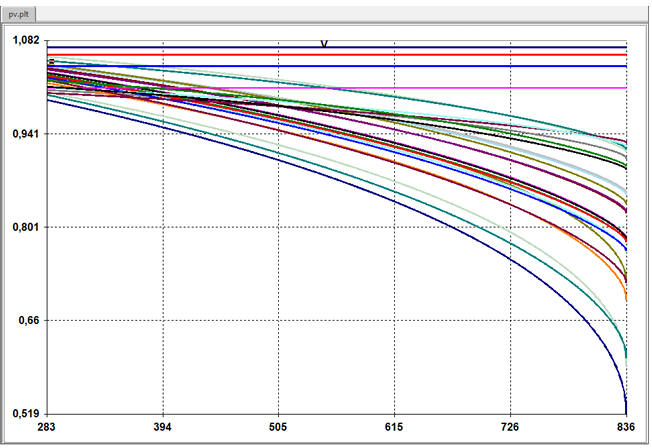
\includegraphics[width=\linewidth]{figures/curva_pv_madureira_ref.png}
    \caption{Reference ANAREDE PV trajectory \cite{madureira2023avaliacao}.}
    \label{fig:curvapv_ref}
\end{figure}

\subsection{Convergence Analysis and Final State}

The convergence history illustrates the operation of the adaptive step-refinement mechanism. As the boundary is approached, increments that previously converged become infeasible and the step is repeatedly reduced. At the final converged state, Bus 30 reached 0.5029 pu with a voltage angle of $-79.83^\circ$, while the electrically adjacent Bus 29 reached 0.5769 pu. The concentration of the voltage degradation in this area indicates that the limiting condition is associated with the inability to sustain the required power transfer to the remote load region.

\subsection{Comparative Analysis of Indices (IEEE 30-Bus)}

All five VSIs were calculated over the stored loadability trajectory. The first objective of this comparison is to determine whether the different formulations identify the same stressed branches and buses. The second is to evaluate how rapidly their values evolve as the system approaches the MLP.

Figure~\ref{fig:indices_fvsi} presents FVSI. The index increases strongly on a restricted group of branches, particularly Lines 1, 2, and 4, indicating increasing reactive-transfer stress near the generation outlets.

\begin{figure}[!t]
    \centering
    
\includegraphics[width=\linewidth]{figures/analise_fvsi_30.pdf}
    \caption{Evolution of FVSI along the IEEE 30-bus loading trajectory.}
    \label{fig:indices_fvsi}
\end{figure}

The $L_{mn}$ results in Fig.~\ref{fig:indices_lmn} provide a similar spatial diagnosis. The most stressed elements are again emphasized, and critical values above 0.8 occur in the high-loading region. The similarity is expected because both formulations depend strongly on branch reactance, reactive transfer, and sending-end voltage.

\begin{figure}[!t]
    \centering
    
\includegraphics[width=\linewidth]{figures/analise_lmn_30.pdf}
    \caption{Evolution of the $L_{mn}$ index along the loading trajectory.}
    \label{fig:indices_lmn}
\end{figure}

NLSI, shown in Fig.~\ref{fig:indices_nlsi}, includes both active and reactive receiving-end power. Its response remains strongly related to FVSI and $L_{mn}$ but provides a somewhat broader differentiation among highly loaded branches.

\begin{figure}[!t]
    \centering
    
\includegraphics[width=\linewidth]{figures/analise_nlsi_30.pdf}
    \caption{Evolution of NLSI along the IEEE 30-bus loading trajectory.}
    \label{fig:indices_nlsi}
\end{figure}

The NVSI results in Fig.~\ref{fig:indices_nvsi} show a more distinct sensitivity profile. Because the formulation combines receiving-end apparent power with a voltage-dependent denominator, the index can grow differently from the other branch-oriented metrics as the voltage level deteriorates.

\begin{figure}[!t]
    \centering
    
\includegraphics[width=\linewidth]{figures/analise_nvsi_30.pdf}
    \caption{Evolution of NVSI along the IEEE 30-bus loading trajectory.}
    \label{fig:indices_nvsi}
\end{figure}

Finally, Fig.~\ref{fig:indices_lindex} presents the nodal L-Index. In contrast with the previous metrics, the L-Index does not rank transmission branches. It identifies vulnerable load buses through the global network admittance relationship and therefore provides complementary information on the location of the weakest voltage region.

\begin{figure}[!t]
    \centering
    
\includegraphics[width=\linewidth]{figures/analise_l_index_30.pdf}
    \caption{Nodal L-Index evolution for the IEEE 30-bus system.}
    \label{fig:indices_lindex}
\end{figure}

\subsection{VSI Statistical Correlation Analysis}

A Spearman rank-correlation analysis was used to quantify similarity among the four branch-oriented VSIs at the limiting operating condition. Spearman's coefficient is suitable because the objective is to compare the ordering of critical branches rather than assume a linear relation between absolute index values.

Table~\ref{tab:spearman} shows an almost perfect correlation between FVSI and $L_{mn}$ ($\rho_s=0.9962$). NLSI is also strongly correlated with FVSI and $L_{mn}$, with coefficients of 0.9024 and 0.9181, respectively. NVSI provides a more distinct ordering, with correlations of 0.4228 with FVSI, 0.4578 with $L_{mn}$, and 0.6200 with NLSI. These results indicate that FVSI and $L_{mn}$ provide largely redundant branch-ranking information in this case, while NVSI contributes a less similar response.

\begin{table}[!t]
\centering
\caption{Spearman Correlation Between Branch-Based VSIs}
\label{tab:spearman}
\begin{tabular}{lcccc}
\toprule
 & FVSI & $L_{mn}$ & NLSI & NVSI \\
\midrule
FVSI     & 1.0000 & 0.9962 & 0.9024 & 0.4228 \\
$L_{mn}$& 0.9962 & 1.0000 & 0.9181 & 0.4578 \\
NLSI     & 0.9024 & 0.9181 & 1.0000 & 0.6200 \\
NVSI     & 0.4228 & 0.4578 & 0.6200 & 1.0000 \\
\bottomrule
\end{tabular}
\end{table}

The L-Index is intentionally excluded from this table because it is defined over buses rather than branches. A direct spatial rank correlation between these two domains would require an additional branch-to-bus mapping and could obscure the different physical interpretation of the metrics. Its contribution is therefore evaluated qualitatively as a nodal complement to the branch indices.

\subsection{N-1 Contingency Analysis and Ranking}

The intact-network loadability margin does not necessarily represent the most restrictive condition faced during operation. For this reason, the framework was extended to N-1 line contingencies. Each transmission line is removed individually, the post-contingency state is recalculated, and the loadability search is repeated. In these contingency cases, generator reactive-power limits are enforced through PV-to-PQ conversion when the available reactive reserve is exhausted.

Contingency severity is ranked through the resulting $\lambda_{\max}$: a lower value indicates that the post-contingency system reaches its loading boundary sooner. Table~\ref{tab:n1_ranking} lists the ten most severe line outages. Line 9 is the most restrictive event, reducing $\lambda_{\max}$ to 2.0140. Lines 0 and 37 are the next most severe contingencies, with $\lambda_{\max}$ equal to 2.1920 and 2.4580, respectively.

\begin{table}[!t]
\centering
\caption{Ten Most Severe N-1 Line Contingencies}
\label{tab:n1_ranking}
\begin{tabular}{cc}
\toprule
\textbf{Line} & $\bm{\lambda_{\max}}$ \\
\midrule
9  & 2.0140 \\
0  & 2.1920 \\
37 & 2.4580 \\
1  & 2.5631 \\
3  & 2.5919 \\
6  & 2.6420 \\
24 & 2.6580 \\
36 & 2.6640 \\
5  & 2.6980 \\
34 & 2.7160 \\
\bottomrule
\end{tabular}
\end{table}

The ranking demonstrates that a single component outage can substantially reduce the available loading margin compared with the intact-network baseline. It also highlights the importance of combining voltage-stability monitoring with contingency-aware operating conditions. The baseline case remains useful for validating the model and understanding the unconstrained transfer limit, whereas the N-1 results provide a more restrictive perspective when topology changes and reactive limits are considered.

\subsection{Application and Comparison: IEEE 39-Bus System}
To evaluate how network topology impacts the predictive capacity of stability indices, the same CPF algorithm was applied to the IEEE 39-bus New England system. Unlike the 30-bus network, which presents radial-like weak corridors, the 39-bus system is heavily meshed and supported by a larger number of generation units. This evaluation serves to test the algorithm's standalone robustness without directly comparing it to ANAREDE.

\textbf{1. PV Curve Behavior and Stability Margin:}
While the IEEE 30-bus system showed a steep, distinct ``nose'' curve for its weakest bus (\autoref{fig:curvapv}), the PV curves generated for the IEEE 39-bus system exhibited a more uniform and gradual voltage degradation across multiple load buses prior to collapse. The strong meshing allowed active power to be rerouted efficiently, pushing the Maximum Loading Point (MLP) to a significantly higher load margin. Specifically, the system safely evolved from a base load of 6,254.23 MW to an impressive collapse threshold of 13,357.13 MW ($\bm{\lambda} = 2.1357$), representing a load increase capability of over 113.5\%. At the bifurcation point, Bus 6 was identified as the critical node, reaching a minimum voltage of 0.6629 pu.

\begin{figure}[htbp]
    \centering
    \includesvg[width=\linewidth]{outputs/ieee_39_barras_new_england/pv_figures/curva_pv_sistema_39}
    \caption{PV curves of the IEEE 39-bus New England system, demonstrating a more uniform and resilient voltage degradation profile due to its highly meshed topology.}
    \label{fig:curvapv_39}
\end{figure}

The robustness of the developed backtracking algorithm was heavily tested in this meshed topology. The convergence report indicates that the simulation required 581 iterations to reach the singularity, dynamically reducing the increment step size from an initial $0.2000$ pu down to a highly precise $0.0008$ pu in the final divergent iterations. This ensures the MLP was pinpointed with exact precision rather than a premature numerical divergence.

\textbf{2. Response of Line Indices (FVSI, $L_{mn}$, NLSI, NVSI):}
As previously shown, in the IEEE 30-bus system, line indices saturated quickly and presented sharp spikes near generation outlet lines. Conversely, when calculated for the IEEE 39-bus system (\autoref{fig:indices_fvsi_39}, \autoref{fig:indices_lmn_39}, \autoref{fig:indices_nlsi_39}, \autoref{fig:indices_nvsi_39}), the exact same indices displayed a much broader distribution of stress. 

\begin{figure}[htbp]
    \centering
    \includesvg[width=\linewidth]{outputs/ieee_39_barras_new_england/index_figures/analise_fvsi_39}
    \caption{Evolution of the FVSI line index in the IEEE 39-bus system, showcasing how meshed topologies distribute reactive stress across multiple transmission corridors.}
    \label{fig:indices_fvsi_39}
\end{figure}

\begin{figure}[htbp]
    \centering
    \includesvg[width=\linewidth]{outputs/ieee_39_barras_new_england/index_figures/analise_lmn_39}
    \caption{Progression of the $L_{mn}$ line index in the IEEE 39-bus system, reflecting a distributed burden rather than localized bottlenecks.}
    \label{fig:indices_lmn_39}
\end{figure}

\begin{figure}[htbp]
    \centering
    \includesvg[width=\linewidth]{outputs/ieee_39_barras_new_england/index_figures/analise_nlsi_39}
    \caption{Response of the NLSI line index to loading increments, highlighting shared transmission burdens across the IEEE 39-bus grid.}
    \label{fig:indices_nlsi_39}
\end{figure}

\begin{figure}[htbp]
    \centering
    \includesvg[width=\linewidth]{outputs/ieee_39_barras_new_england/index_figures/analise_nvsi_39}
    \caption{Evolution of the NVSI index in the IEEE 39-bus system, illustrating the distributed impact of apparent power variations.}
    \label{fig:indices_nvsi_39}
\end{figure}

Rather than a few lines peaking abruptly, multiple interconnected components experienced a simultaneous, gradual rise in their index values. The power flow report near the collapse point corroborates this, revealing severe and distributed loading across critical corridors, such as Transformer 2-9 (242.8\% loaded) and Line 21-15 (201.6\% loaded). This demonstrates that in highly meshed networks, line indices may be less effective at pinpointing a single point of failure, as the network tends to distribute the burden and collapse holistically rather than locally.

\textbf{3. Response of Nodal Indices (L-Index):}
In contrast to the line indices, the L-Index proved to be consistently reliable across both topologies. Just as it correctly identified the weakest node in the 30-bus network, the L-Index successfully highlighted the most vulnerable load buses in the 39-bus system (\autoref{fig:indices_lindex_39}) as it approached the MLP, demonstrating its analytical robustness regardless of grid meshing. It is important to note that buses connected to generators were not considered in this index.

\begin{figure}[htbp]
    \centering
    \includesvg[width=\linewidth]{outputs/ieee_39_barras_new_england/index_figures/analise_l_index_39}
    \caption{Nodal vulnerability mapping using the L-Index in the complex IEEE 39-bus topology, maintaining predictive accuracy regardless of grid meshing.}
    \label{fig:indices_lindex_39}
\end{figure}

\section{Conclusions}
\label{sec:conclusions}

This work presented an open-source Python framework for static voltage-stability assessment using a step-refined loadability search and five established VSIs. The IEEE 30-bus model was cross-compared with ANAREDE and reached an MLP of 809.69 MW, corresponding to a 185.71\% increase relative to the 283.40 MW base load and a 3.15\% deviation from the 836 MW reference result. The voltage trajectory identifies Bus 30 as the weakest region near the loading boundary.

The VSI analysis showed that the branch-oriented indices do not provide independent information. FVSI and $L_{mn}$ are almost perfectly rank-correlated, while NLSI also preserves a strong association with both. NVSI produces a more distinct branch ranking and therefore adds complementary sensitivity within the line-based group. The L-Index should be interpreted separately because it evaluates buses through the global admittance relationship rather than ranking transmission branches.

The N-1 study further demonstrated that the intact-network margin is insufficient to characterize the most restrictive condition. When line outages and generator reactive-power limits are considered, the available loadability can decrease substantially; among the analyzed outages, Line 9 produced the lowest $\lambda_{\max}$. These results support a combined methodology in which the loadability boundary provides the reference for system stress, VSIs provide element-level monitoring information, and contingency analysis identifies operating conditions that can reduce the available margin. The numerical values remain dependent on the adopted load-growth direction, generation redispatch, reactive-power limits, transformer settings, and power-flow convergence criteria.

\bibliographystyle{IEEEtran}
\bibliography{refs}

\end{document}
